%\documentclass[a4paper,german,10pt]{tumarticle}
\documentclass[a4paper,english,10pt]{tumarticle}

\usepackage[utf8]{inputenc}
\usepackage{tumfonts}
\usepackage{tumlocale}
\usepackage{tumcmd}
\usepackage{booktabs}
\usepackage{eurosym}
\usepackage{enumitem}
\usepackage{subfig}
\usepackage[font=footnotesize,labelfont=bf]{caption}
\usepackage[hidelinks]{hyperref}
\usepackage{wrapfig}
\usepackage{pgfgantt}
\usepackage{adjustbox}
\usepackage{pdflscape}
\usepackage{hyperref}
\usepackage{listings}
\lstset{ 
  backgroundcolor=\color{white},
  breakatwhitespace=false,
  breaklines=true,
  frame=single,
  keepspaces=true,
  keywordstyle=\color{blue},
  language=Python,
  numbers=left,
  numbersep=5pt,
  rulecolor=\color{black},
  showspaces=false,
  showstringspaces=false,
  showtabs=false,
}

\usetikzlibrary{decorations.text}

\usepackage{siunitx}
\sisetup{detect-weight=true, detect-family=true, per-mode=symbol}
\DeclareSIUnit\year{a}
\DeclareSIUnit{\EUR}{\text{EUR}}
\DeclareSIUnit{\week}{Woche}

\def\yes{\textcolor{TUMDarkerGreen}{\large\checkmark}}
\def\maybe{\textcolor{TUMOrange}{\Large$\mathbit\circ$}}
\def\no{\textcolor{TUMRed}{\Large\texttimes}}

% Set document title. If no language is supplied, the document language is
% assumed.

\linespread{1.32}
%\predisplaypenalty=10000000
%\floatingpenalty = 20000000
%\postdisplaypenalty = 2000000
\widowpenalty=15000
\setlength{\parindent}{0pt}



\begin{document}

\begin{center}
	\bfseries\Large Validation Tool for \texttt{libmoeprlnc}\\[.5\baselineskip]
\end{center}
\begin{center}
	\small Group 6\\
	\today
\end{center}


\setcounter{tocdepth}{1}
\renewcommand{\contentsname}{Anlagen}
%\begin{tableofcontents}
%\end{tableofcontents}

\renewcommand{\emph}[1]{%
	\textcolor{TUMBlue}{#1}%
}


% Motivation und Abstract
\renewcommand{\abstractname}{Abstract}
\begin{abstract}
\setlength{\parindent}{0pt}
\noindent%
\footnotesize

This project proposes a validating tool for the \texttt{libmoeprlnc} library. 
\\TODO:\\
//TODO: Außerdem konnte die lib per statistischer auswertung validert werden\\
//TODO: und es konnten die folgenden bugs gefunden werden...

\end{abstract}

\section{Introduction}

The \texttt{libmoeprlnc} library implements the encoding and decoding of generations in
random linear network coding. It is based on the \texttt{libmoepgf} library, which in turn
implements the required Galois Field operations.

The \texttt{libmoeprlnc} (also referred to as \texttt{rlnc library} in the following) does not yet have an 
adequate testing suit. Our group proposes a validation tool for the \texttt{rlnc library} which mainly tries to 
find unexpected bugs by executing the libraries functions in a random order.

In addition to bugs in the code that might lead to a crash, we have also made it our task to check the functionality 
of the library by means of statistical evaluations.

This paper documents of the proposed tool, as well as the results of our evaluation.

\section{Approach}\label{app}

\subsection{Brief Description of the \texttt{rlnc library}}\label{app:desc}
The following will briefly describe the functionality of the main interfaces, the \texttt{rlnc library} offers.
This is required to better understand the proposed approach by this project.
\\\\
First of all, the library uses a data structure called \texttt{rlnc\_block} which is the libraries representation of a generation.
Since our tool also has an abstraction of a generation, in the following the term "rlnc\_block" describes this libraries data structure and 
"generation" the abstraction of our tool. Besides this data structure, the library offers four main interfaces: 
\texttt{rlnc\_block\_add()}, \texttt{rlnc\_block\_encode()}, \texttt{rlnc\_block\_decode()} and \texttt{rlnc\_block\_get()}.

\begin{itemize}
    \item \underline{\texttt{rlnc\_block\_add(rlnc\_block\_t b, int pv, const uint8\_t *data, size\_t len)}}\\
    Reads the data of size \texttt{len} from \texttt{*data} and add it to the \texttt{rlnc\_block} \texttt{b}. Pivot (\texttt{pv}) describes the index of the data in the generation. 
    (TODO @Tobi ist das richtig mit dem pivot?). 

    \item \underline{\texttt{rlnc\_block\_encode(const rlnc\_block\_t b, uint8\_t *dst, size\_t maxlen, int flags)}}\\
    Encodes data from the \texttt{rlnc\_block} \texttt{b} pseudo randomly (TODO: drauf eingehen warum das 'pseudo' hier wichtig sein könnte) and returns the coded data at \texttt{*dst}. 
    \texttt{maxlen} describes the aligned length of the buffer \texttt{dst}. The alignment is chosen at the initialization of the \texttt{rlnc\_block}.
    
    \item \underline{\texttt{rlnc\_block\_decode(rlnc\_block\_t b, const uint8\_t *src, size\_t len)}}\\
    Receives coded data in \texttt{src} which is of length \texttt{len} and adds it to \texttt{rlnc\_block} \texttt{b}. 
    Then the \texttt{rlnc\_block} is decoded as far as possible. 
    Consequently, any linear dependencies that may have arisen are eliminated in this step. If the rank(b) should 
    be equal to the generation size after the execution of this method, the holder of \texttt{b} can now read the fully decoded generation.

    \item \underline{\texttt{rlnc\_block\_get(rlnc\_block\_t b, int pv, uint8\_t *dst, size\_t maxlen)}}\\
    If the requested data has already been decoded, the function returns the data of \texttt{rlnc\_block} \texttt{b} at index \texttt{pv} in buffer 
    \texttt{dst} of size \texttt{maxlen} (aligned).
  \end{itemize}

\subsection{Building the Tool}\label{app:build}
TODO: Dependencies + build-steps... Also wsl. einfach README reinkopieren. 

\subsection{The Tool and Its Program Flow}\label{sec:tool}
Generally, our tool simulates the communication between two partners A and B. 
A holds a Generation containing randomly generated bytes. Using the \texttt{rlnc library}, A transmits coded information to B. 
During this process, coded data might be lost with a user-defined probability. When B receives the coded information, 
it adds it to its own \texttt{rlnc\_block} and tries to decode it. Decoded data might then be consumed and added to the Generation B.
An iteration was successful exactly if Generation A and B contain the same data at the end.

There are checks distributed in the code, that verify whether return values are as expected or 
the library itself throws errors. If there is an an unexpected behavior detected or the library itself returns an error, 
the tool terminates and outputs what happened.

To simulate the presented communication flow, our tool mainly introduces the following three function:

create\_at\_A() extracts the next frame from Generation A and adds it to the underlying \texttt{rlnc\_block}. 

transmit\_A2B() represents a transmission between A and B. Therefore, coded data is generated from the 
\texttt{rlnc\_block} which is held by A (if the block is not empty). Then, the coded data might either be 'lost' 
with the user-defined loss probability (the function returns without further actions)
or it is added to the \texttt{rlnc\_block} held by B. By adding coded data to a \texttt{rlnc\_block} the library will try to decode the block as far as possible
and therefore eliminate any linear dependencies that might have been added to the \texttt{rlnc\_block B}.

consume\_at\_B() represents the consumption of decoded data on the B side. 
The tool tries to read the next available decoded data and (if available) adds it to the Generation B.

For better clarity of the flow of data, all three functions are shown in Figure \ref{fig:func}.

\begin{figure}[h]
  \center
  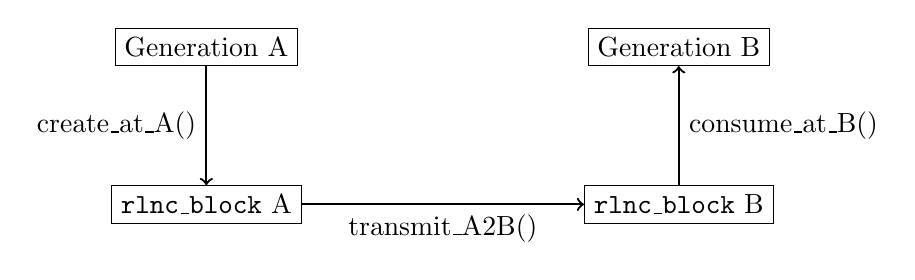
\begin{tikzpicture}
    \node[draw] at (0, 2)   (ga) {Generation A};
    \node[draw] at (0, 0)   (ba) {\texttt{rlnc\_block} A};
    \node[draw] at (6, 2)   (gb) {Generation B};
    \node[draw] at (6, 0)   (bb) {\texttt{rlnc\_block} B};
    \draw [thick,->] (ga) -- (ba) node[midway,left] {create\_at\_A()};
    \draw [thick,->] (ba) -- (bb) node[midway,below] {transmit\_A2B()};
    \draw [thick,->] (bb) -- (gb) node[midway,right] {consume\_at\_B()};
  \end{tikzpicture}
  \caption{Data Flow}
  \label{fig:func}
\end{figure}

During the whole process, our tool mainly distinguishes between two modes that strongly influence the program flow. 
The random mode and the prefill mode mode. 
The idea behind the random mode is basically a random execution of the interfaces provided by the library under test, 
to especially detect bugs that occur only in very rare edge cases.
In general, the prefill mode is more deterministic and is better suited for 
statistical analysis for various reasons, which will be explained in more detail below.

During the execution of the program, various information relevant for a statistical evaluation can be collected and output in a CSV file.

\subsubsection{The random mode}\label{sec:random}
During an iteration in random mode, the tool repeatedly chooses one of the three functions, introduced in Section \ref{sec:tool}, 
to be called, each with probability $\frac{1}{3}$. 

This way, it is possible to randomly generate numerous scenarios, when testing enough iteration. 
Especially edge-case scenarios like the following ones are tested:

\begin{itemize}
  \item \texttt{rlnc\_block B} is still empty and we try to read decoded frames from it.
  \item \texttt{rlnc\_block A} is empty and the program tries to generate coded data from it and transmit it.
  \item \texttt{rlnc\_block A} is only partly filled and the program already starts transmitting.
\end{itemize}

\subsubsection{The prefill mode}\label{sec:prefill}
However, the random mode comes with some challenges if one wants to make meaningful and reliable statistical 
evaluations of the program output.

As mentioned in the introduction of Section \ref{sec:tool}, an iteration ends when generation A and B contain the same data. 
However, in random mode it may happen that the \texttt{rlnc\_block} already contains all required information but due
to the random nature of the mode, the consuming function might not be called immediately.
Since we are often interested in how many transmissions it took at a minimum for B to decode the whole generation, this behavior 
might distort the number of required transmissions, especially in an nondeterministic way.

furthermore the random mode tries to send already coded data while the \texttt{rlnc\_block} on the A side has not been completely filled yet. 
This of course leads to the fact that the probability for sending linearly dependent packets is very high at the beginning and 
decreases with time. 
To solve the described problems we built the prefill mode.

The prefill mode fills the complete \texttt{rlnc\_block} of the A side at the beginning and transmits until the 
\texttt{rlnc\_block} of the B side has full rank. Then all packets are consumed at once and it is checked 
whether generation A and B contain the same data.

\subsection{Command Line Parameters}\label{app:cmd}
TODO update parameters\\
Our proposed tool accepts the following command line parameters:

\begin{itemize}
    \item -c, \texttt{-{}-}csv\_stats\\
    Print statistics to CSV file in current working directory.

    \item -f, \texttt{-{}-}field\_size=SIZE\\
    Set underlaying Galois Field size. (0: GF2, 1: GF4, 2: GF16, 3: GF256).

    \item -g, \texttt{-{}-}gen\_size=SIZE\\
    Set the generation size.

    \item -i, \texttt{-{}-}nr\_iterations=ITER\\
    Set the amount of test iterations

    \item -l, \texttt{-{}-}loss\_rate=LOSS\\
    Set probability with which a coded packet is lost during transmission.

    \item -p, \texttt{-{}-}pkt\_size=SIZE (TODO frame size??)\\
    Set the packet size.

    \item -s, \texttt{-{}-}seed=ADDR\\
    Set the seed which is used to generate random test input.
    \item -v, \texttt{-{}-}verbose

    Produce verbose output.
\end{itemize}

\section{Evaluation}\label{sec:eval}
According to the lecture, the probability that N randomly chosen coding vectors form
the complete N-dimensional vector space is given by equation \ref{eq:decode_prob}.
\begin{equation} 
  Pr[dim\bigcup_{i=1}^{N}\{c_i\} = N] = \prod_{i=1}^{N} (1 - \frac{q^{i - 1}}{q ^ {N}})
  \label{eq:decode_prob}
\end{equation}

Where N is the generation size and q the size of the underlying Galois Field ($q \in \{2,4,16,256\}$).

Applied to the context of our project, equation \ref{eq:decode_prob} gives us the probability that the 
\texttt{rlnc\_block} \texttt{b} can be completely decoded after exactly N transmissions.

TODO: Darauf eingehen, warum der seed die auswertung beeinflusst und warum wir in die library eingreifen mussten.\\
TODO: Hier grafiken und statistische Auswertungen.


\section{Validation of our Tool}\label{eval}
TODO: Jonas meinte ja dass wir irgendwie zumindest im Ansatz unser Tool auch validieren sollen. 

\section{Conclusion}\label{eval}
In this project, a tool for validating the \texttt{libmoeprlnc} was implemented, presented and successfully used 
to validate the library. 

During the entire working phase, no profound bugs could be identified.

In particular, the expected decoding probability presented in the lecture 
could also be verified in Section \ref{sec:eval}, which is another indication of the correctness of the library.

During the development only by an error of our side it was noticed that the method rlnc\_block\_decode() does not 
throw an error, although it gets a buffer with coded data, which is smaller than the data length defined 
at initialization. However, since coded data consists of the linear combination of data of the same length and 
the respective coding vector, the case described above should never occur.

Consequently, we suggest that the method should throw an error in this case. In all other methods, 
the library already shows such behavior and throws an error if an illogical buffer size is passed.

TODO: Irgendwo erwähnen, dass wir den random mode sehr viel haben laufen lassen und keinen Fehler feststellen konnten


\end{document}